

\begin{frame}[plain]
\frametitle{Summary: structural transition in CeSb$_2$}
\hspace{5em}{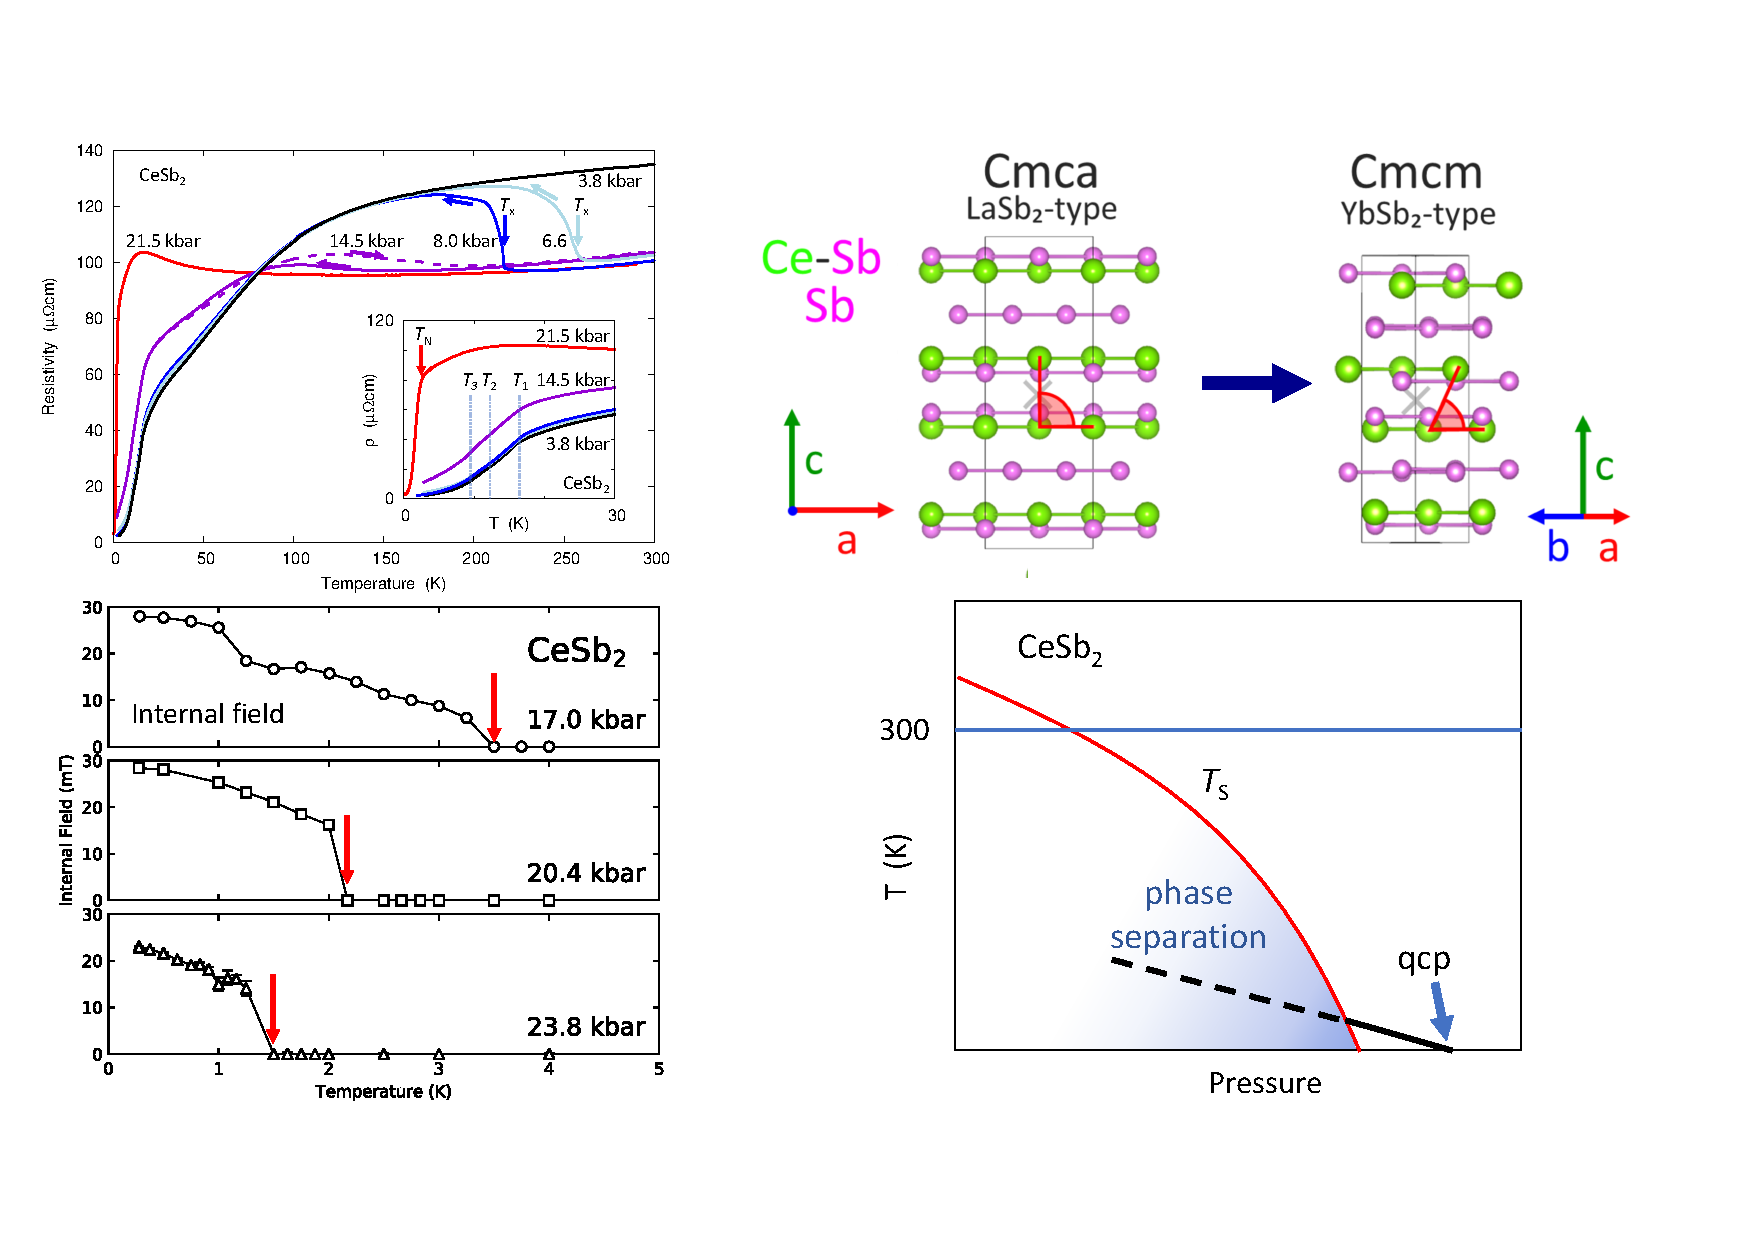
\includegraphics[width=1.2\columnwidth]{EndingPicture1}}
%\vspace{-1em}
%\begin{center}
% Soft modes are built into some quasiperiodic structures. \\
  \mbox{\small Pressure-induced structural transition $\rightarrow$ correlated, magnetic high pressure state. }
%\end{center}
% \vspace*{\fill}
% \centerline{\makebox[\linewidth]{\rule{0.85\textwidth}{0.4pt}}}
% \centerline{\scriptsize P. Brown Sci. Adv. (2018)}
\end{frame}


%%% Local Variables: 
%%% mode: latex
%%% TeX-master: "GroTalk"
%%% End: 
